\PassOptionsToPackage{table}{xcolor}
\documentclass[12pt,letterpaper,twocolumn,openany,nodeprecatedcode,bg=none]{dndbook}
\usepackage[english]{babel}
\usepackage[utf8]{inputenc}
\usepackage{longtable,booktabs,array}
\usepackage{calc}
\usepackage{etoolbox}
\usepackage{caption}
\usepackage{float}
\usepackage{graphicx}
\usepackage{needspace}
\usepackage{tikz}

% Reset zebra striping at the start of every table
\AtBeginEnvironment{longtable}{\rowcolors{1}{white}{gray!10}\small}
\AtBeginEnvironment{table}{\rowcolors{1}{white}{gray!10}}

\providecommand{\pandocbounded}[1]{#1}
\providecommand{\tightlist}{%
  \setlength{\itemsep}{0pt}\setlength{\parskip}{0pt}}

\captionsetup{labelformat=empty}
\setcounter{secnumdepth}{0}
\setlength{\parindent}{0pt}
\setlength{\parskip}{0.5\baselineskip}
\setlength{\headheight}{15pt}

% Prevent orphaned subsections
\let\oldsubsection\subsection
\renewcommand{\subsection}[1]{%
  \needspace{5\baselineskip}%
  \oldsubsection{#1}%
}

\begin{document}
\onecolumn

      \title{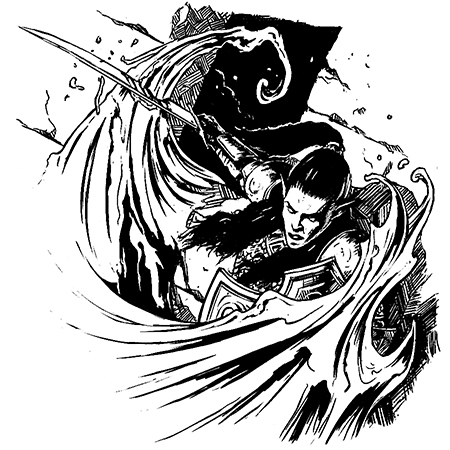
\includegraphics[width=0.9\textwidth,height=0.55\textheight,keepaspectratio]{elfPaladin.jpg}\\[1.5cm]Arcane
Knight}
  \author{Class Handbook}
\date{}
\maketitle

\clearpage
\thispagestyle{empty}
\null\vfill
\begin{center}{\Large\itshape Your trusty class handbook for fantasy
gaming.}\end{center}
\vfill

\clearpage
\thispagestyle{empty}
\begin{center}
\vspace*{\fill}
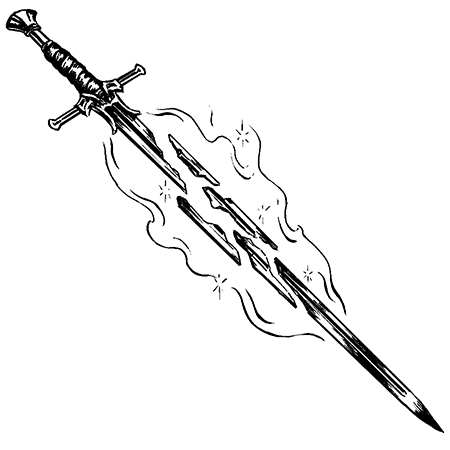
\includegraphics[width=\textwidth,height=0.85\textheight,keepaspectratio]{magicSword.jpg}\par
\vspace{0.4cm}
{\itshape Nothing makes a hero more than reforging an ancient magic
sword.}\par
\vspace*{\fill}
\end{center}

\clearpage
\twocolumn

\section{Arcane Knight}\label{arcane-knight}

\subsection{Core Arcane Knight Traits}\label{core-arcane-knight-traits}

\needspace{11\baselineskip}

{\def\LTcaptype{none} % do not increment counter
\begin{table}[!htbp]
\centering
\begin{tabular}{@{}
  >{\raggedright\arraybackslash}p{(\linewidth - 2\tabcolsep) * \real{0.4483}}
  >{\raggedright\arraybackslash}p{(\linewidth - 2\tabcolsep) * \real{0.5517}}@{}}
\toprule\noalign{}
\begin{minipage}[b]{\linewidth}\raggedright
\textbf{Primary Ability}
\end{minipage} & \begin{minipage}[b]{\linewidth}\raggedright
Strength
\end{minipage} \\
\midrule\noalign{}
\textbf{Hit Points} & 1d6 \\
\textbf{Saving Throw Proficiencies} & Strength, Intelligence, Wisdom \\
\textbf{Skill Proficiencies} & Choose 2 skills \\
\textbf{Weapon Proficiencies} & Choose 3 categories \\
\textbf{Starting Equipment} & Greatsword, Scale Mail, Grimoire \\
\bottomrule\noalign{}
\end{tabular}
\end{table}
}

\subsection{Arcane Knight Features}\label{arcane-knight-features}

\needspace{20\baselineskip}

{\def\LTcaptype{none} % do not increment counter
\begin{table}[!htbp]
\centering
\begin{tabular}{@{}
  >{\raggedright\arraybackslash}p{(\linewidth - 4\tabcolsep) * \real{0.1020}}
  >{\raggedright\arraybackslash}p{(\linewidth - 4\tabcolsep) * \real{0.2245}}
  >{\raggedright\arraybackslash}p{(\linewidth - 4\tabcolsep) * \real{0.6735}}@{}}
\toprule\noalign{}
\begin{minipage}[b]{\linewidth}\raggedright
Level
\end{minipage} & \begin{minipage}[b]{\linewidth}\raggedright
Proficiency
\end{minipage} & \begin{minipage}[b]{\linewidth}\raggedright
Class Features
\end{minipage} \\
\midrule\noalign{}
1 & +2 & Spellcasting, Enchanted Weapon \\
2 & +2 & --- \\
3 & +2 & Ability Bonus \\
4 & +2 & --- \\
5 & +2 & Two Attacks \\
6 & +2 & --- \\
7 & +2 & Ability Bonus, Mighty Enchantment \\
8 & +2 & --- \\
9 & +3 & --- \\
10 & +3 & --- \\
\bottomrule\noalign{}
\end{tabular}
\end{table}
}

\subsection{Level 1: Spellcasting}\label{level-1-spellcasting}

You can cast spells from the Arcane Knight spell list. Wisdom is your
casting ability. You know zero cantrips.

You prepare a number of spells equal to your total number of spell
slots. You may change your prepared spells after an extended period of
downtime.

You regain all expended spell slots when you finish a long rest. Once
per day, you may regain 1 expended spell slot when you finish a short
rest.

\subsection{Spell Slots by Level}\label{spell-slots-by-level}

\needspace{20\baselineskip}

{\def\LTcaptype{none} % do not increment counter
\begin{table}[!htbp]
\centering
\begin{tabular}{@{}
  >{\raggedright\arraybackslash}p{(\linewidth - 6\tabcolsep) * \real{0.3571}}
  >{\raggedright\arraybackslash}p{(\linewidth - 6\tabcolsep) * \real{0.2143}}
  >{\raggedright\arraybackslash}p{(\linewidth - 6\tabcolsep) * \real{0.2143}}
  >{\raggedright\arraybackslash}p{(\linewidth - 6\tabcolsep) * \real{0.2143}}@{}}
\toprule\noalign{}
\begin{minipage}[b]{\linewidth}\raggedright
Level
\end{minipage} & \begin{minipage}[b]{\linewidth}\raggedright
1
\end{minipage} & \begin{minipage}[b]{\linewidth}\raggedright
2
\end{minipage} & \begin{minipage}[b]{\linewidth}\raggedright
3
\end{minipage} \\
\midrule\noalign{}
1 & 2 & -- & -- \\
2 & 2 & -- & -- \\
3 & 3 & -- & -- \\
4 & 3 & -- & -- \\
5 & 4 & 2 & -- \\
6 & 4 & 2 & -- \\
7 & 4 & 3 & -- \\
8 & 4 & 3 & -- \\
9 & 4 & 3 & 2 \\
10 & 4 & 3 & 2 \\
\bottomrule\noalign{}
\end{tabular}
\end{table}
}

\subsection{Level 1: Enchanted Weapon}\label{level-1-enchanted-weapon}

Pick a weapon that you have enchanted with your battle magic. You roll
an additional 1d4 when rolling the weapon's damage.

\subsection{Level 3: Ability Bonus}\label{level-3-ability-bonus}

You gain a +1 bonus to two different abilities of your choice.

\subsection{Level 5: Two Attacks}\label{level-5-two-attacks}

When you attack, you can make two weapon attacks.

\subsection{Level 7: Ability Bonus}\label{level-7-ability-bonus}

You gain a +1 bonus to two different abilities of your choice.

\subsection{Level 7: Mighty
Enchantment}\label{level-7-mighty-enchantment}

If the d4 you roll for Enchanted Weapon rolls a 4, roll an additional
1d4. Repeat this process for the extra dice granted by this feature.

\subsection{Arcane Knight Spells}\label{arcane-knight-spells}

The tables are numbered for random spell selection. This class has no
cantrips listed.

\subsubsection{Level 1 Spells}\label{level-1-spells}

\needspace{9\baselineskip}

{\def\LTcaptype{none} % do not increment counter
\begin{table}[!htbp]
\centering
\begin{tabular}{@{}
  >{\raggedright\arraybackslash}p{(\linewidth - 2\tabcolsep) * \real{0.1765}}
  >{\raggedright\arraybackslash}p{(\linewidth - 2\tabcolsep) * \real{0.8235}}@{}}
\toprule\noalign{}
\begin{minipage}[b]{\linewidth}\raggedright
d4
\end{minipage} & \begin{minipage}[b]{\linewidth}\raggedright
Level 1
\end{minipage} \\
\midrule\noalign{}
1 & Bless \\
2 & Cure Wounds \\
3 & Detect Magic \\
4 & Inflict Wounds \\
\bottomrule\noalign{}
\end{tabular}
\end{table}
}

\subsubsection{Level 2 Spells}\label{level-2-spells}

\needspace{9\baselineskip}

{\def\LTcaptype{none} % do not increment counter
\begin{table}[!htbp]
\centering
\begin{tabular}{@{}
  >{\raggedright\arraybackslash}p{(\linewidth - 2\tabcolsep) * \real{0.1500}}
  >{\raggedright\arraybackslash}p{(\linewidth - 2\tabcolsep) * \real{0.8500}}@{}}
\toprule\noalign{}
\begin{minipage}[b]{\linewidth}\raggedright
d4
\end{minipage} & \begin{minipage}[b]{\linewidth}\raggedright
Level 2
\end{minipage} \\
\midrule\noalign{}
1 & Augury \\
2 & Restorative Touch \\
3 & Silence \\
4 & Zone of Truth \\
\bottomrule\noalign{}
\end{tabular}
\end{table}
}

\subsubsection{Level 3 Spells}\label{level-3-spells}

\needspace{9\baselineskip}

{\def\LTcaptype{none} % do not increment counter
\begin{table}[!htbp]
\centering
\begin{tabular}{@{}
  >{\raggedright\arraybackslash}p{(\linewidth - 2\tabcolsep) * \real{0.1667}}
  >{\raggedright\arraybackslash}p{(\linewidth - 2\tabcolsep) * \real{0.8333}}@{}}
\toprule\noalign{}
\begin{minipage}[b]{\linewidth}\raggedright
d4
\end{minipage} & \begin{minipage}[b]{\linewidth}\raggedright
Level 3
\end{minipage} \\
\midrule\noalign{}
1 & Dispel Magic \\
2 & Remove Curse \\
3 & Revivify \\
4 & Speak with Dead \\
\bottomrule\noalign{}
\end{tabular}
\end{table}
}

\newpage

\section{Arcane Knight Spell List}\label{arcane-knight-spell-list}

Spells descriptions are listed below.

\subsection{Augury}\label{augury}

\textbf{Level:} 2

You receive an omen from mystical forces about the results of a course
of action that you plan to take within the next 30 minutes. The DM
chooses whether to answer weal, woe, or a mix of the two, depending on
the most likely outcome of the action.

\subsection{Bless}\label{bless}

\textbf{Level:} 1

\textbf{Range:} 30 feet

\textbf{Duration:} Concentration, up to 1 minute

You bless up to three creatures within range. A blessed creature adds
1d4 to their attack rolls and saves.

\subsection{Cure Wounds}\label{cure-wounds}

\textbf{Level:} 1

\textbf{Range:} Touch

A creature you touch regains 2d8 + your spellcasting bonus hit points.

The healing increases to 4d8 + your spellcasting bonus if you use a
level 2 slot and 6d8 + your spellcasting bonus if you use a level 3
slot.

\subsection{Detect Magic}\label{detect-magic}

\textbf{Level:} 1

\textbf{Range:} Self

\textbf{Duration:} Concentration, up to 10 minutes

You see the presence of magical effects within 30 feet on objects that
are visible to you. Magic appears as a faint aura, the details of which
allow you to determine its origin and the basic details of its effect.

\subsection{Dispel Magic}\label{dispel-magic}

\textbf{Level:} 3

\textbf{Range:} 120 feet

Choose one creature, object, or magical effect within range. Any ongoing
spell of level 3 or lower on the target ends. For each ongoing spell of
level 4 or higher on the target, make an ability check using your
spellcasting ability (DC 10 plus that spell's level). On a successful
check, the spell ends.

\subsection{Inflict Wounds}\label{inflict-wounds}

\textbf{Level:} 1

\textbf{Range:} Touch

A creature you touch makes a Constitution saving throw, taking 2d10
Necrotic damage on a failed save or half damage on a successful one.

The damage increases to 4d10 Necrotic damage if you use a level 2 slot
and 6d10 Necrotic damage if you use a level 3 slot.

\newpage

\subsection{Remove Curse}\label{remove-curse}

\textbf{Level:} 3

\textbf{Range:} Touch

At your touch, all curses affecting one creature or object end. If the
object is a cursed magic item, its curse remains, but the spell allows
the owner to remove or discard it.

\subsection{Restorative Touch}\label{restorative-touch}

\textbf{Level:} 2

\textbf{Range:} Touch

You touch a creature and end one condition on it: blinded, paralyzed, or
poisoned.

\subsection{Revivify}\label{revivify}

\textbf{Level:} 3

\textbf{Range:} Touch

You touch a creature. If that creature died within the last minute, it
returns to life, restores one failed death save, and regains 1 hit
point. It cannot restore failed death saves again until it finishes a
long rest.

\subsection{Silence}\label{silence}

\textbf{Level:} 2

\textbf{Range:} 120 feet

\textbf{Duration:} Concentration, up to 10 minutes

No sound can be created within or pass through a 20-foot-radius sphere
centered on a point you choose within range. Any creature or object
entirely inside the sphere has immunity to thunder damage. Spells cannot
be cast in the spell's area.

\subsection{Speak with Dead}\label{speak-with-dead}

\textbf{Level:} 3

\textbf{Range:} 10 feet

\textbf{Duration:} 10 minutes

You touch a corpse and attempt to commune with its spirit. If its spirit
can be contacted, you contact it through mystical means.

Until the spell ends, you can ask the spirit of the corpse up to five
questions. The spirit knows only what it knew in life, including the
languages it knew. The spirit is under no compulsion to offer a truthful
answer if you are antagonistic toward it or it recognizes you as an
enemy.

The dead often demand a service in return for the information they
provide. If you accept such a deal, you cannot cast this spell again
until you complete the task or make a good faith effort to do so.

\subsection{Zone of Truth}\label{zone-of-truth}

\textbf{Level:} 2

\textbf{Range:} 60 feet

\textbf{Duration:} 10 minutes

You create a magical zone that guards against deception in a
15-foot-radius sphere centered on a point within range. A creature that
enters the spell's area for the first time on a turn or starts its turn
there makes a Charisma saving throw. On a failed save, a creature can't
speak a deliberate lie while in the radius. You know whether a creature
succeeds or fails on this save.

An affected creature is aware of the spell and can avoid answering
questions to which it would normally respond with a lie. Such a creature
can be evasive yet must be truthful.

\onecolumn

\clearpage
\thispagestyle{empty}
\begin{center}
\vspace*{\fill}
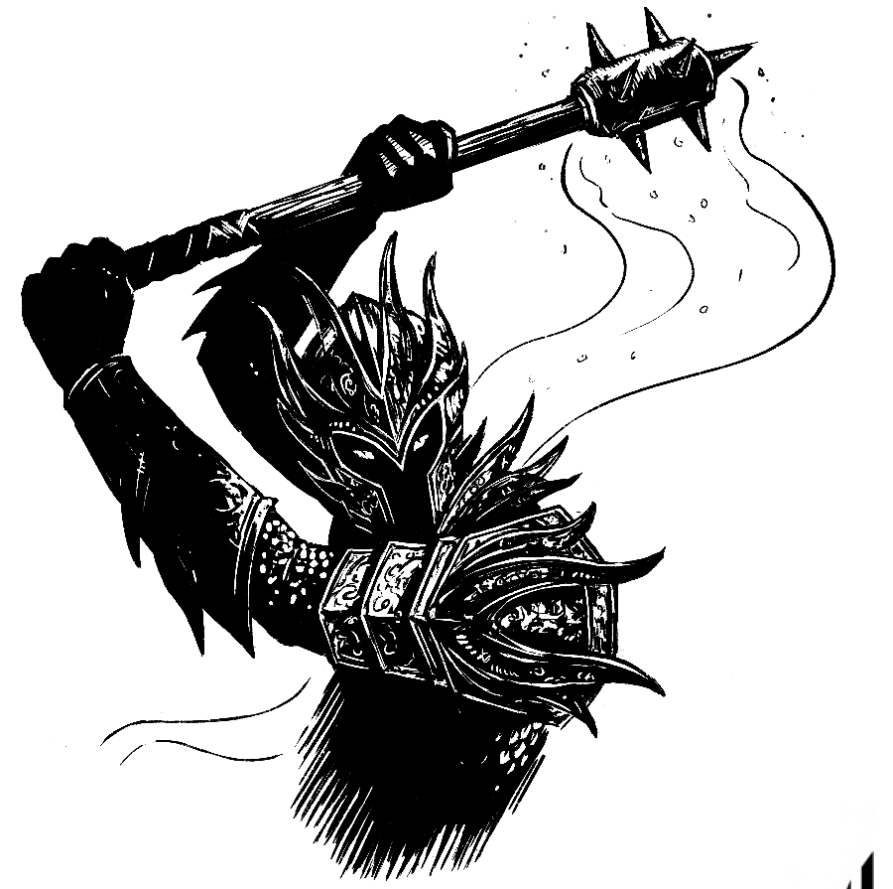
\includegraphics[width=0.7\textwidth,keepaspectratio]{deathKnight.png}\par
\vspace{0.4cm}
{\itshape An arcane knight wields all forms of power.}\par
\vspace*{\fill}
\end{center}

\end{document}